This section will introduction a recursive formula of the Weil--Petersson volume by integrate McShane--Mirzakhani identity(\ref{McMiid}) over  the moduli space $\mathscr{M}_{g,n}(L)$ using theorem \ref{integrformu}. The result is that the Weil--Petersson volume of $\mathscr{M}_{g,n}(L)$ is a polynomial of $L_1^2,\cdots,L_n^2$. Assume $n>0$ in this section, since for $n=0$ the Weil--Petersson volume only depends on $g$. The hyperbolic condition requires  that $2g-2+n>0$.

\begin{theorem}\label{poly}
Define $V_{g,n}(L)$ to be the Weil--Petersson volume of $\mathscr{M}_{g,n}(L)$, then 
\begin{equation}\label{polyeq}
    V_{g,n}(L)=\sum\limits_{|\alpha|\leq 3g-3+n}c_\alpha L^{2\alpha}.
\end{equation}
Here $c_\alpha>0$, $\frac{c_\alpha}{\pi^{6g-6+2n-2|\alpha|}}\in \mathbb{Q}$, and for $\alpha=(\alpha_1,\cdots,\alpha_n)$, $L^{2\alpha}=L_1^{2\alpha_1}\cdots L_n^{2\alpha_n}$. In particular, the coefficients of those leading terms in $V_{g,n}(L)$  are rational.
\end{theorem}


Define some auxiliary functions as follows:

Set $L=(L_1,\cdots,L_n)$ and $\hat{L}=(L_2,\cdots,L_n)$, for $(g,n)\neq (1,1),(0,3)$,
then define 
\begin{equation}\label{Acon}
A_{g,n}(L)=\frac{1}{2}\int_0^\infty\int_0^\infty xy\hat{A}_{g,n}(x,y,L)dxdy,
\end{equation}

\begin{equation}\label{Adcon}
    A_{g,n}^{d}(L)=\frac{1}{2}\int_0^\infty\int_0^\infty xy\hat{A}_{g,n}(x,y,L)dxdy,
\end{equation}

\begin{equation}\label{Bfor}
    B_{g,n}(L)=\int_0^\infty x\hat{B}_{g,n}(x,L)dx,
\end{equation}
with the functions  $\hat{A}_{g,n},\hat{A}_{g,n}^{d},\hat{B}_{g,n}$ defined later.

Fix $$m(g,n)=\delta(g-1)\times \delta(n-1),$$ with $\delta$ the Dirac function with value $1$ at $0$ and value $0$ at other point. It represents whether $S_{g,n}$ is a $S_{1,1}$.

\begin{remark}
The notation $d$ for $A_{g,n}^{d}$ means  it calculates for the case that $S_{g,n}-P$  is discontinuous, while   for $A_{g,n}$ it calculates the case that $S_{g,n}-P$  is continuous, where $P$ is a pair of pants with one boundary component $\beta_1$. 

In  these formulas, $L_1$ is not equivalent with $L_i$, $i\geq 2$, While $L_i$ and $L_j$ are equivalent with $i,j\geq2$, here the equivalence means the commutation of the values of them won't change the values of these functions. so one may write $L=(L_1,\hat{L})$ with $\hat{L}=(L_2,\cdots,L_n)$.
\end{remark}

\begin{definition}[ $\hat{A}_{g,n}$]
$$
\hat{A}_{g,n}(x,y,L_1,\hat{L})=\frac{1}{2^{m(g-1,n+1)}}V_{g-1,n+1}(x,y,\hat{L})H(x+y,L_1).
$$
\end{definition}

\begin{definition}[$\hat{B}_{g,n}$]
$$
\begin{aligned}
\hat{B}_{g,n}=&(x,L_1,\hat{L})=\frac{1}{2^{m(g,n-1)}}\sum_{j=2}^n\frac{1}{2}(H(x,L_1+L_j)+H(x,L_1-L_j))\\
\times & V_{g,n-1}(x,L_2,\cdots,\hat{L_j},\cdots,L_n)\\
\end{aligned}
$$
\end{definition}

\begin{definition}[$\hat{A}_{g,n}^{d}$]
Define the index set  $I_{g,n}$ as the set of ordered  pairs 
$((g_1,I_1),(g_2,I_2))$ with $$I_1\sqcup I_2=\{2,3,\cdots,n\}, 2\leq n_i+2g_i,g_1+g_2=g,$$
where $|I_i|=n_i$, $g_i\geq 0$. Here the notation $\sqcup$ means the disjoint union.

For $I=\{i_1,\cdots i_k\}\subset \{2,3\cdots,n\}$,  set $$
L_I=(L_{i_1},\cdots,L_{i_k}),
$$
then define $\hat{A}_{g,n}^{d}$ by 
$$
\begin{aligned}
&\hat{A}_{g,n}^{d}(x,y,L)=\sum_{I_{g,n}}H(x+y,L_1)\\
&\times \frac{V_{g_1,n_1+1}(x,L_{I_1})}{2^{m(g_1,n_1+1)}}\times  \frac{V_{g_2,n_2+1}(x,L_{I_2})}{2^{m(g_2,n_2+1)}}\\
\end{aligned}
$$


\end{definition}

These functions will be helped to deal with  the Weil--Petersson volume $V_{g,n}(L)$ for $2g-2+n>0$.


\begin{theorem}
Assume that $(g,n)\neq(1,1),(0,3)$, then 
the recursion formula of  $V_{g,n}(L)$ is given by the following identity:
\begin{equation}\label{recursivefor}
    \frac{\partial }{\partial L_1}(L_1V_{g,n}(L))=A_{g,n}(L)+A_{g,n}^{d}(L)+B_{g,n}(L).
\end{equation}
\end{theorem}

\begin{proof}
By (\ref{McMiid}),  $$\sum_{\{\gamma_1,\gamma_2\}\in F_1}D(L_1,l_{\gamma_1} (X),l_{\gamma_2}(X))+\sum_{i=2}^n\sum_{\gamma\in  F_{1,i}}R(L_1,L_i,l_{\gamma}(X))=L_1.$$

Define $$
    \mathscr{D}(X)=\sum\limits_{\{\gamma_1,\gamma_2\}\in F_1}D(L_1,l_{\gamma_1} (X),l_{\gamma_2}(X)),
$$
 $$
    \mathscr{R}_i(X)=\sum_{\gamma\in  F_{1,i}}R(L_1,L_i,l_{\gamma}(X)),
$$


To take advantage of Mirzakhani's integration formula, it will be helpful to write $\mathscr{D}$ and $\mathscr{R}_i$ in the form of $f_\gamma$, where $f$ is some function defined on the moduli space and $\gamma$ is some multi-curve. 

Notice that $\Mod_{g,n}$ acts on $F_{1,i}$ transitively, since $\gamma$ and $\eta$ are on the same orbits of the $\Mod_{g,n}$  action if and only if there is a heomeomorphism from $S_{g,n}(\gamma)$ to $S_{g,n}(\eta)$ which fixes the $n$ boundary components $\{\beta_i\}_{i=1}^n$ of $S_{g,n}$, and both $\gamma,\eta$ will cut $S_{g,n}$ into $S_{0,3}$ and $S_{g,n-1}$. Then for fixed $i$,
set $\gamma_i\in F_{1,i}$ to be  an arbitrary element, and the function $R^i(x)=R(L_1,L_i,x)$, then $$
\begin{aligned}
R_{i,\gamma_i}(x)=&\sum_{\gamma\in \Mod_{g,n}\ \cdot \gamma_i}R_i(l_\gamma(X))\\
=&\sum_{\gamma\in F_{1,i}} R(L_1,L_i,l_{\gamma}(X))\\
=&\mathscr{R}_i(X).\\
\end{aligned}
$$

Apply theorem \ref{integrformu}, then $M(\gamma_i)=1$ if and only if the $S_{g,n-1}$ part is $S_{1,1}$, so $M(\gamma_i)=m(g,n-1)$ , and $|\sym(\gamma_i)|=1$, $N(\Gamma)=1$  so 
$$
\begin{aligned}
&\int_{\mathscr{M}_{g,n}(L)}\mathscr{R}_i(X)dX\\
=&\frac{1}{1\cdot 2^{m(g,n-1)}}\int_0^\infty xR(L_1,L_i,x)  \mathrm{Vol}(\mathscr{M}_{g,n}(\Gamma,x,\beta,L))x\cdot dx\\
=&\frac{1}{2^{m(g,n-1)}}\int_0^\infty xR(L_1,L_i,x)\frac{1}{1}V_{g,n-1}(x,L_2,\cdots,\hat{L_i},\cdots,L_n)dx.\\
\end{aligned}
$$
Take the derivation with respect to $L_1$, by (\ref{pp2}),
$$
\frac{\partial }{\partial L_1}R(L_1,L_i,x)=\frac{1}{2}(H(x,L_1-L_j)+H(x,L_1+L_j)),
$$
then \begin{equation}\label{partialL1}
    \sum_i\frac{\partial }{\partial L_1}\int_{\mathscr{M}_{g,n}(L)}\mathscr{R}_i(X)dX=B_{g,n}(L).
\end{equation}

\begin{figure}[h]
    \centering
    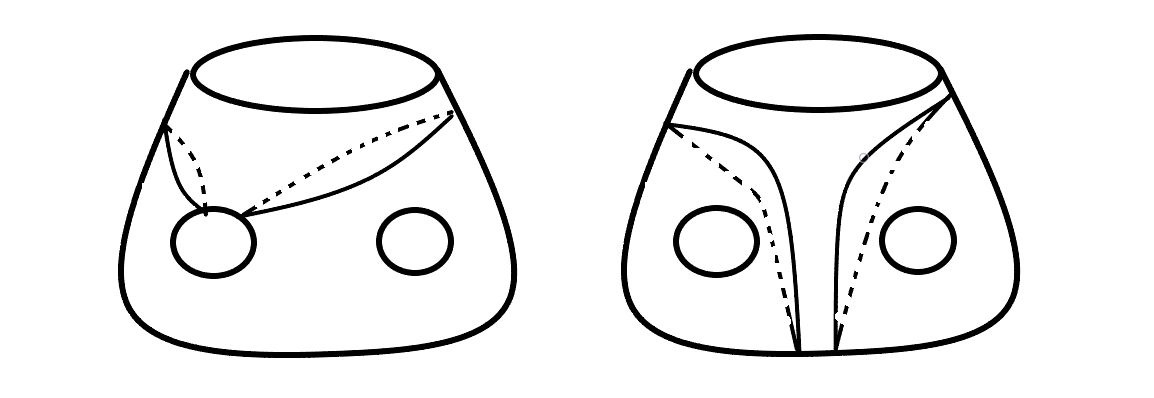
\includegraphics[width=3 in]{picture/gammatype.png}
    \caption{An example for different types of $\gamma_1+\gamma_2\in F_1$}
    \label{fig:gammatype}
\end{figure}

While for $\{\gamma_1,\gamma_2\}$ in $F_{1}$, the type of $\gamma=\gamma_1+\gamma_2$ is determined by the separated surface  $S_{g,n}(\gamma)$. Figure \ref{fig:gammatype} is an example of $\gamma=\gamma_1+\gamma_2$  of different types in $F_1$.
 
Set $\Sigma_{\gamma_1,\gamma_2}$ to be the pair of pants bounded by $\beta_1,\gamma_1,\gamma_2$.
Notice that if $S_{g,n}-\Sigma_{\gamma_1,\gamma_2}$ is not connected, then $S_{g,n}(\gamma)$ is the union of $S_{0,3}$ and $S_{g-1,n+1}$.  If $S_{g,n}-\Sigma_{\gamma_1,\gamma_2}$ is disconnected, then  $S_{g,n}-\Sigma_{\gamma_1,\gamma_2}$ contains two parts $S_{g_1,n_1}$ and $S_{g_2,n_2}$, with  $n_1+n_2=n+1$, and $g_1+g_2=g$. Here the conditions for genus are both  from the Gauss--Bonnet theorem, which shows that  $Vol(S_{g,n})=-2\pi\Chi(S_{g,n})=2\pi(2g-2+n)$.

 By the same argument as for $F_{1,i}$,  let $S\subset F_{1}$ be the set of unordered pair $(\gamma_1,\gamma_2)$ with $S_{g,n}-\Sigma_{\gamma_1,\gamma_2}$ connected, Then $\Mod_{g,n}$ acts transitively on $S$. Take $\gamma=\gamma^0_1+\gamma^0_2$ with $(\gamma_1^0,\gamma_2^0)\in S$, and fix $D_S(x)=D(L_1,x,0)$. Notice that by (\ref{D}),$$\begin{aligned}
D(x,y,z)=&2\log \left(\frac{e^{\frac{x}{2}}+e^{\frac{y+z}{2}}}{e^{\frac{-x}{2}}+e^{\frac{y+z}{2}}}\right)\\
=&D(x,y+z,0),\\
\end{aligned}$$
then $$\begin{aligned}
D_\gamma(x)&=\sum_{(\gamma_1,\gamma_2)\in S}D(L_1,l_{\gamma_1+\gamma_2}(X),0)\\
=&\sum_{(\gamma_1,\gamma_2)\in S}D(L_1,l_{\gamma_1}(X),l_{\gamma_2}(X)).\\
\end{aligned}$$

Apply theorem \ref{integrformu}, notice that $M(\gamma)=m(g-1,n+1)$, $|\sym(\gamma)|= 2$, and $N(\gamma)=1$, then 
$$
\begin{aligned}
&\int_{\mathscr{M}_{g,n}(L)}D_\gamma(X)dX\\
=&\frac{1}{2\cdot 2^{m(g-1,n+1)}}\int_0^\infty \int_0^\infty  xyD(L_1,x+y,0)  \mathrm{Vol}(\mathscr{M}_{g,n}(\Gamma,(x,y),\beta,L))xy\cdot dxdy\\
=&\frac{1}{2}\int_0^\infty\int_0^\infty xy  \frac{1}{2^{m(g-1,n+1)}}D(L_1,x+y,0)\frac{1}{1}V_{g-1,n+1}(x,y,L_2,\cdots,L_n)dxdy.\\
\end{aligned}
$$

Take the derivation with respect to $L_1$, by (\ref{pp1}),
$$
\frac{\partial }{\partial L_1}D(L_1,x+y,0)=H(x+y,L_1),
$$
thus \begin{equation}\label{partialL2}
   \sum_{(\gamma_1,\gamma_2)\in S} \frac{\partial }{\partial L_1}\int_{\mathscr{M}_{g,n}(L)}D(L_1,l_{\gamma_1}(X),l_{\gamma_2}(X))dX=A_{g,n}(L).
\end{equation}

Notice that these arguments hold for $g\geq 1$. If $g=0$ then this term vanishes, since $F_{1}$ is empty. By the same time, $A_{g,n}=0$, $A_{g,n}^{d}=0$ if $g=0$. Then for arbitrary $g$ the formula holds.


For $a=((g_1,I_1),(g_2,I_2))\in I_{g,n}$, Take $S_a=\{(\gamma_1,\gamma_2)\in F_1|S_{g,n}-\Sigma_{\gamma_1,\gamma_2}=S_{g_1,n_1+1}\cup S_{g_2,n_2+1}\}$. Then $\Mod_{g,n}$ acts transitively on $S_a$ for each $a\in I_{g,n}$.

Take $\gamma_a=\gamma_1^a+\gamma_2^a$, with $(\gamma_1,\gamma_2)\in S_a$, then 
$$\begin{aligned}
D_{\gamma_a}(x)&=\sum_{(\gamma_1,\gamma_2)\in S_a}D(L_1,l_{\gamma_1+\gamma_2}(X),0)\\
=&\sum_{(\gamma_1,\gamma_2)\in S_a}D(L_1,l_{\gamma_1}(X),l_{\gamma_2}(X)).\\
\end{aligned}$$

 Apply theorem \ref{integrformu}, notice that $M(\gamma_a)=m(g_1,n_1+1)+m(g_2,n_2+1)$, $|\sym(\gamma_a)|= 2$ if $n=1$ and $g_1=g_2$ since elements in $\Mod_{g,n}$ fix the boundary components, $|\sym(\gamma_a)|=1$ otherwise.  
 $N(\gamma)=1$. Then 
$$
\begin{aligned}
&\int_{\mathscr{M}_{g,n}(L)}D_{\gamma_a}(X)dX\\
=&c_a\cdot \int_0^\infty \int_0^\infty  xyD(L_1,x+y,0)  \mathrm{Vol}(\mathscr{M}_{g,n}(\Gamma,(x,y),\beta,L))xy\cdot dxdy\\
=&c_a^\prime\cdot\int_0^\infty\int_0^\infty xy  \frac{1}{2^{m(g-1,n+1)}}D(L_1,x+y,0)\frac{1}{1}
V_a(x,y,L)
dxdy.\\
\end{aligned}
$$
where $$c_a=\frac{1}{2^{\delta_{g_1}(g_2)\cdot \delta(n-1)}\cdot 2^{m(g_1,n_1+1)+m(g_2,n_2+1)}},$$ $$c_a^\prime=\frac{1}{2^{\delta_{g_1}(g_2)\cdot \delta(n-1)}},$$ and $$V_a(x,y,L)=\frac{V_{g_1,n_1+1}(x,L_{I_1})}{2^{m(g_1,n_1+1)}}\frac{V_{g_2,n_2+1}(y,L_{I_2})}{2^{m(g_2,n_2+1)}}.$$

Since $\cup_{a\in I_{g,n}}S_a=F_1\backslash S$,add it  over $F_1\backslash S$ and take the derivation with respect to $L_1$, then 
\begin{equation}\label{partialL3}
\begin{aligned}
   &\sum_{(\gamma_1,\gamma_2)\in F_1\backslash S} \frac{\partial }{\partial L_1}\int_{\mathscr{M}_{g,n}(L)}D(L_1,l_{\gamma_1}(X),l_{\gamma_2}(X))dX \\
   =&\frac{1}{2}\int_0^\infty \int_0^\infty H(x+y,L_1)V_a(x,y,L)dxdy =A_{g,n}^{d}(L).\\
   \end{aligned}
\end{equation}


Notice that if $n=1$ and $g_1=g_2$, then $c_\alpha^\prime=\frac{1}{2}$, otherwise, $a=((g_1,I_1),(g_2,I_2))$ and $b=((g_2,I_2),(g_1,I_1))$ correspond to the same subset $S_a=S_b\subset F_{1}$, so in the summation it needs to multiply the factor $\frac{1}{2}$.

Combine (\ref{partialL1}), (\ref{partialL2}), (\ref{partialL3}) and (\ref{McMiid}), then (\ref{recursivefor}) follows.
\end{proof}


For the case of $(g,n)=(1,1),(0,3)$, the Weil--Petersson volume can be computed  directly.

By lemma \ref{uni}, $\mathscr{M}_{0,3}(L)$ consists only one element, so $V_{0,3}(L_1,L_2,L_3)=1$.

For $V_{1,1}(L)$, it is also followed by the Mirzakhani's integration formula, and the McShane--Mirzakhani identity degenerates to 
$$
\sum_{\gamma\in F_{1}}D(L,l_\gamma(X),l_\gamma(X))=L,
$$
where $F_1$ is the set of all simple closed geodesics.  $Mod_{1,1}$ acts transitively on $F_1$ by the component of Dehn twists and half twists. Define $D(x)=D(L,x,x)$, then 
$$
D_\gamma(X)=\sum_{\gamma\in F_1}D(L,l_\gamma(X),l_\gamma(X)).
$$
Integrate it over $\mathscr{M}_{1,1}(L)$ and apply theorem \ref{integrformu}, $N(\gamma)=2$, $|\sym(\gamma)|=1$, $M(\gamma)=1$,
then 
$$\begin{aligned}
    \int_{\mathscr{M}_{1,1}(L)}L_1dX
    =&\frac{1}{1}\int_0^\infty xD(L,x,x)\frac{1}{2}\cdot 1\cdot dx,\\
    \end{aligned}
$$
so $$\begin{aligned}
&\frac{\partial }{\partial L}(L\cdot V_{1,1}(L))=
\frac{1}{2}\int _0^\infty x(\frac{1}{1+e^{x+\frac{L}{2}}}+\frac{1}{1+e^{x-\frac{L}{2}}})dx\\
=&\frac{1}{2}\int_{\frac{L}{2}}^\infty \frac{x-\frac{L}{2}}{1+e^{x}}dx+\frac{1}{2}\int_{-\frac{L}{2}}^\infty \frac{x+\frac{L}{2}}{1+e^{x}}dx\\
=&\int_{0}^\infty\frac{x}{1+e^x}dx+\frac{1}{2}\int_0^{\frac{L}{2}}(\frac{L}{2}-x)(\frac{1}{1+e^x}+\frac{1}{1+e^{-x}})dx\\
=&\int_{0}^\infty\frac{x}{1+e^x}dx+\frac{L^2}{16}.\\
\end{aligned}
$$
While $$\begin{aligned}
&\int_{0}^\infty \frac{x}{1+e^x}dx 
=\sum_{k=0}^\infty \int_0^\infty(-1)^kxe^{-(k+1)x}dx\\
=&\sum_{k=0}^\infty(-1)^k\frac{1}{(k+1)^2}
=\sum_{k=1}^\infty \frac{1}{k^2}-2\sum_{k=1}^\infty\frac{1}{(2k)^2}\\
=&\frac{\pi^2}{12},\\
\end{aligned}
$$
so
$$
\frac{\partial }{\partial L}(L\cdot V_{1,1}(L))=\frac{\pi^2}{12}+\frac{L^2}{16},
$$
thus $$V_{1,1}(L)=\frac{\pi^2}{12}+\frac{L^2}{48}.$$

\begin{remark}
Due to historical reason, when $Vol(\mathscr{M}_{1,1}(L))$ is needed in  Mirzakhani's integration  formula, it is $\frac{1}{24}(L^2+4\pi^2)$ for the existence of  $M(\gamma)$.
\end{remark}

Now $V_{0,3}(L)$ and $V_{1,1}(L)$ satisfy the form in $(\ref{polyeq})$, and $\frac{\partial }{\partial L_1}(L_1V_{g,n}(L))=A_{g,n}(L)+A_{g,n}^{d}(L)+B_{g,n}(L).$
If $A_{g,n}(L)$, $A_{g,n}^{d}(L)$, $B_{g,n}(L)$ are both polynomials of $L_1^2,\cdots,L_n^2$ of the form $\sum_{|\beta|\leq 3g-3+n}c_\beta L^{2\beta}$ with $c_\beta\in \pi^{6g-6+2n-2|\beta|}\cdot \mathbb{Q}$, then so does $V_{g,n}(L)$.

\begin{definition}
For $i\in \mathbb{N}$, set $$
F_{2i+1}=\int_0^\infty x^{2i+1}H(x,t)dt.
$$
\end{definition}

\begin{lemma}\label{Fzeta}
For a positive integer $i$,
\begin{equation}
    F_{2i+1}(t)=(2i+1)!\sum_{j=0}^{i+1}\zeta(2j)(2^{2j+1}-4)\frac{t^{2i+2-2j}}{(2i+2-2j)!}.
\end{equation}
In particular, $F_{2i+1}(t)=\sum_{j=0}^{i+1}c_j^i t^{2j},$ with $c_j^i\in \pi^{2i+2-2j}\cdot\mathbb{Q}$, and $c_{i+1}^i=\frac{1}{2i+2}$.
\end{lemma}

\begin{proof}
Notice that $$
\begin{aligned}
n^{-s}\Gamma(s)=&\int_0^\infty (\frac{x}{n})^{s}e^{-x}\frac{dx}{x}\\
=&\int_0^\infty x^{s-1}e^{-nx}dx,\\
\end{aligned}
$$
so $$
\begin{aligned}
\zeta(s)\Gamma(s)=&\sum_{n=1}^\infty\int_0^\infty x^{s-1}e^{-nx}dx\\
=&\int_0^\infty \frac{x^{s-1}}{e^x-1}dx.
\end{aligned}
$$
Moreover, $\Gamma(k)=(k-1)!$ for integer $k>0$ and $$\begin{aligned}
&\int_0^\infty \frac{x^{k}}{1+e^x}dx \\
=&\int_0^\infty x^k(\frac{e^x+1-2}{e^{2x}-1})dx\\
=&\int_0^\infty \frac{x^k}{e^x-1}dx-2\int_0^\infty \frac{x^k}{e^{2x}-1}dx\\
=&\int_0^\infty \frac{x^k}{e^x-1}dx(1-2^{-k}).\\
\end{aligned}
$$
As a result, $$
\int_0^\infty \frac{x^k}{1+e^k}dx=\zeta(k+1)\Gamma(k+1)(1-2^{-k}).
$$
Then we can see $$
\begin{aligned}
F_{2i+1}(t)=&\int_0^\infty x^{2i+1}(\frac{1}{1+e^{(x+t)/2}}+\frac{1}{1+e^{(x-t)/2}})dx\\
=&\int_0^\infty \frac{(x+t)^{2i+1}+(x-t)^{2i+1}}{1+e^{x/2}}dx\\
+&\int_0^t(t-x)^{2i+1}(\frac{1}{1+e^{(x-t)/2}}+\frac{1}{1+e^{(t-x)/2}})dx\\
=&\frac{t^{2i+2}}{2i+2}+\int_0^\infty\frac{2\sum_{k=0}^i t^{2k}x^{2i+1-2k}C_{2i+1}^{2k}}{1+e^{x/2}}dx\\
=&\frac{t^{2i+2}}{2i+2}+\int_0^\infty\frac{2\sum_{k=1}^{i+1} t^{2i+2-2k}x^{2k-1}C_{2i+1}^{2k-1}}{1+e^{x/2}}dx\\
=&\frac{t^{2i+2}}{2i+2}+\sum_{k=1}^{i+1} 2C_{2i+1}^{2k-1} t^{2i+2-2k}2^{2k}\int_0^\infty\frac{(x/2)^{2k-1}}{1+e^{x/2}}d\frac{x}{2}\\
=&\frac{t^{2i+2}}{2i+2}+\sum_{k=1}^{i+1}2t^{2i+2-2k}\frac{(2i+1)!}{(2i+2-2k)!}\zeta(2k)(2^{2k}-2)\\
=&\sum_{j=0}^{i+1}\zeta(2j)(2^{2j+1}-4)\frac{t^{2i+2-2j}}{(2i+2-2j)!}\\
\end{aligned}
$$
\end{proof}

\begin{remark}
 $\zeta(0)=-\frac{1}{2},$ and $\zeta(2n)$ is a polynomials of $\pi^{2}$ of degree $n$ with coefficients in  $\mathbb{Q}$.
\end{remark}





\begin{lemma}\label{Fmn}
For integers $n,m\geq 0$,
$$
\int_{0}^Lx^m(L-x)^ndx=\frac{n!m!}{(n+m+1)!}L^{n+m+1}.
$$
\end{lemma}
\begin{proof}
This follows integration by parts.
$$
\begin{aligned}
&\int_0^Lx^m(L-x)^ndx\\
=&\frac{1}{m+1}\int_0^\infty (L-x)^ndx^{m+1}\\
=&\frac{1}{m+1}[(L-x)^nx^{m+1}|_0^L+\int_0^Lx^{m+1}n(L-x)^{n-1}dx]\\
=&\frac{n}{m+1}\int_0^Lx^{m+1}(L-x)^{n-1}dx\\
=&\frac{n(n-1)}{(m+1)(m+2)}\int_0^\infty x^{m+2}(L-x)^{n-2}dx\\
=&\cdots=\frac{n!}{(m+1)\cdots (m+n)}\int_0^\infty x^{m+n}dx\\
=&\frac{n!m!}{(n+m+1)!}L^{n+m+1}.\\
\end{aligned}
$$
\end{proof}
\begin{lemma}\label{xyHint}
\begin{equation}
    \int_{\mathbb{R}_+^2}x^{2p+1}y^{2q+1}H(x+y,t)dxdy=
    \frac{(2p+1)!(2q+1)!}{(2p+2q+3)!}F_{2p+2q+3}(t).
\end{equation}
\end{lemma}
\begin{proof}
Apply lemma \ref{Fmn} and replace $y$ by $z=x+y$,
  $$\begin{aligned}
  &\int_0^\infty\int_0^\infty x^{2p+1}y^{2p+1}H(x+y,t)dxdy\\
  =&\int_0^\infty dz\int_0^zx^{2p+1}(z-x)^{2q+1}H(z,t)dx\\
  =& \frac{(2p+1)!(2q+1)!}{(2p+2q+3)!}\int_0^\infty z^{2p+2q+3}H(z,t)dz\\
  \end{aligned}
  $$
\end{proof}

\begin{proof}[Proof of theorem \ref{poly}]
Notice that in the recursive  formula (\ref{recursivefor}), 
$A_{g,n}(L)$, $A_{g,n}^d(L)$, $B_{g,n}(L)$ rely on   $V_{p,q}(L)$ with $3p+q<3g+n$, thus we can apply the mathematics induction method. 

Suppose (\ref{polyeq}) holds for $(g^\prime,n^\prime)$ with $3g^\prime+n^\prime<3g+n$,  then apply (\ref{Bfor}) and lemma \ref{Fzeta}, $B_{g,n}(L)$ is of the form $\sum_{|\alpha|\leq 3g-3+n}b_\alpha L^{2\alpha}$ with $b_\alpha\in \pi^{6g-6+2n-2|\alpha|}\cdot \mathbb{Q}$.Similarly,  apply (\ref{Acon}), lemma \ref{Fzeta} and lemma \ref{xyHint}, $A_{g,n}(L)$ is of the form $\sum_{|\alpha|\leq 3g-3+n}a_\alpha L^{2\alpha}$ with $a_\alpha\in \pi^{6g-6+2n-2|\alpha|}\cdot \mathbb{Q}$. Apply (\ref{Adcon}), lemma \ref{Fzeta} and lemma \ref{xyHint}, $A_{g,n}^d(L)$ is of the form $\sum_{|\alpha|\leq 3g-3+n}a_\alpha^\prime L^{2\alpha}$ with $a_\alpha^\prime\in \pi^{6g-6+2n-2|\alpha|}\cdot \mathbb{Q}$.
Take them into (\ref{recursivefor}), then theorem \ref{poly} holds for $V_{g,n}(L)$.

Since $V_{1,1}(L)=\frac{\pi^2}{12}+\frac{L^2}{48}$ and $V_{0,3}(L)=1$ have  the desired form $$
V_{g,n}(L)=\sum\limits_{|\alpha|\leq 3g-3+n}c_\alpha L^{2\alpha},
$$
 by the above argument theorem \ref{poly} holds for any pairs $(g,n)$ with $2g-2+n>0$.
\end{proof}